\chapter{Hotel Recognition Accuracy}
\label{ch:5}

Hotels-50K includes a separate test set of images to support the consistent evaluation of 
algorithms. Obtaining a large collection of images from real-world investigations
is problematic for many reasons. However, in the images in the test set are
meant to replicate, as closely as possible the type of data used in these cases.

The test set consists of 17,954 images from the TraffickCam mobile application from 5,000 different 
hotels, which are a subset of those found in the training set. There is no overlap in the 
mobile app users between the training and testing sets to avoid the case of near
duplicates due to multiple images from the same user with the same device captured at the same time.

To replicate real-world conditions where the regions of the image containing victims are 
masked prior to image analysis, the images are augmented with increasingly 
larger "people-shaped" masks. The masks are generated using silhouettes from 'people' regions 
in the MS-COCO semantic labels dataset~\cite{mscoco}. There are four levels of masking (none, low, medium high), corresponding to the relative sizes of the masked region in each image, where the largest masks can occupy up to 85\% of the height of the image. Figure~\ref{fig:example_masks} shows examples of masked test images.

\begin{figure}
    \centering
    % \begin{subfigure}[b]{.45\columnwidth}
    %     \centering
    %     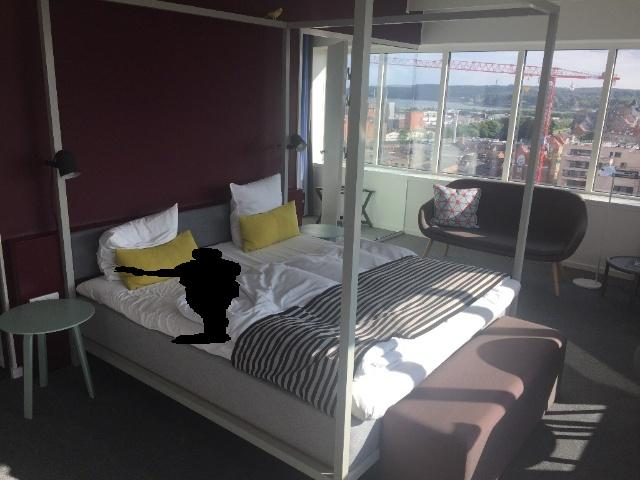
\includegraphics[width=.95\columnwidth]{figures/chapter5/example_masks/0.jpg}
    %  %   \caption{5-25\% occluded}
    % \end{subfigure}
    \begin{subfigure}[b]{.49\columnwidth}
        \centering
        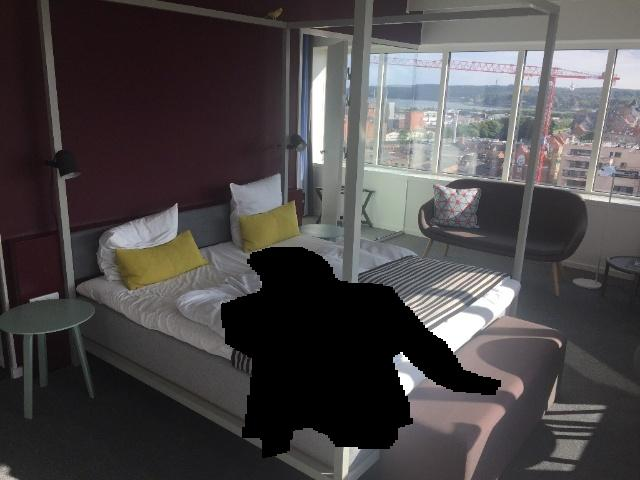
\includegraphics[width=.95\columnwidth]{figures/chapter5/example_masks/1.jpg}
      %  \caption{25-45\% occluded}
    \end{subfigure}
    % \begin{subfigure}[b]{.45\columnwidth}
    %     \centering
    %     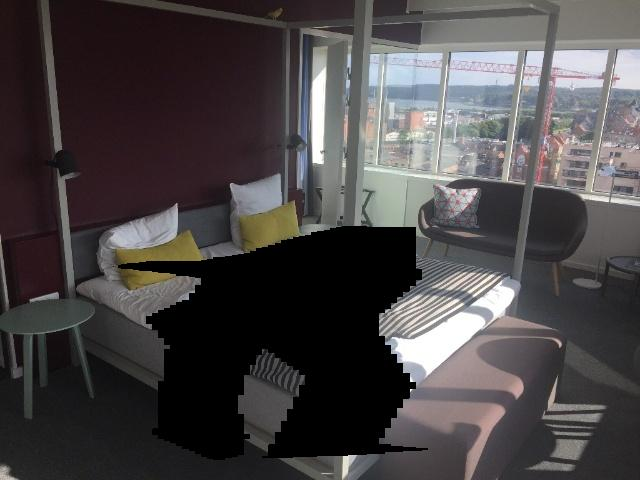
\includegraphics[width=.95\columnwidth]{figures/chapter5/example_masks/2.jpg}
    %   % \caption{45-65\% occluded}
    % \end{subfigure}
    \begin{subfigure}[b]{.49\columnwidth}
        \centering
        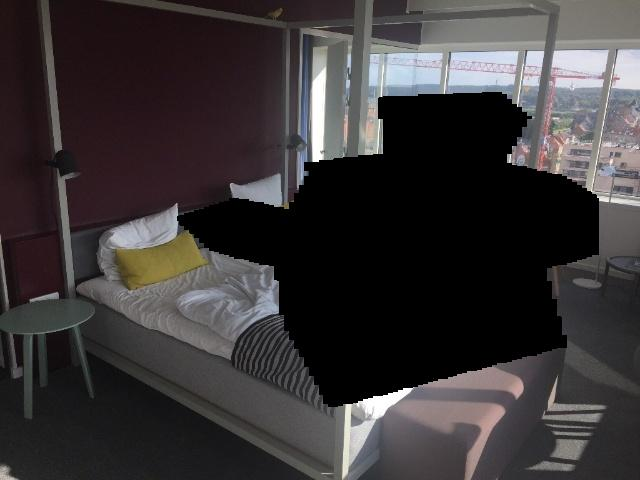
\includegraphics[width=.95\columnwidth]{figures/chapter5/example_masks/3.jpg}
        %\caption{65-85\% occluded}
    \end{subfigure}
    \caption{The images in the test set are augmented with person-shaped masks of varying size.}
    \label{fig:example_masks}
\end{figure}

The evaluation consists of the following tasks:
\begin{description}
\item[Hotel Instance Recognition] The goal for this task is to identify the hotel instance represented for each of the images in the test set.
\item[Hotel Chain Recognition]
The goal for this task is to identify the hotel chain represented in the image. Of 
the test set, 13,136 images are from one of 88 major hotel chains, with the remainder in 
the "Other" category.
\end{description}

\subsection{Evaluation Metrics}
Hotel recognition can be framed as both a classification task (i.e., predict the label given the image) and a retrieval task (i.e., find the most similar database images to a query). The evaluation suite for Hotels-50K supports both variants.

For the retrieval variant, the results should be provided as a
ranked list of the IDs of the 100 most similar images from the Hotels-50K dataset 
to each of the test images. The evaluation metric is top-$K$ accuracy, with $K = \{1, 10, 100\}$ for 
hotel instance recognition and $K = \{1, 3, 5\}$ for hotel chain recognition.

For the classification variant, the results should be provided 
as the posterior probabilities of hotel chains or instances
for each of the test images. The evaluation metrics include the
average multi-class log loss (lower is better) and top-$K$ 
classification accuracy with $K = \{1, 10, 100\}$ for hotel 
instance recognition and $K = \{1, 3, 5\}$ for hotel chain 
recognition.

\section{Results}
In order to set the baseline for performance on the Hotels-50K 
dataset, we compare two "off-the-shelf" pre-trained networks 
trained for object and scene
recognition to a method using data and augmentation schemes specifically tailored to hotel recognition. 

\subsection{Models}
For the pretrained models, we use the fixed feature representations and refer to these as the {\sc Fixed-Object} and {\sc Fixed-Scene} methods. The {\sc Fixed-Object} method is a Resnet-50 network trained on ImageNet (ILSVRC-2012)~\cite{resnet,deng2009imagenet,ILSVRC15}. The feature representation is the 1001-dimensional output from the final fully connected layer. The {\sc Fixed-Scene} method uses a VGG model trained on the Places365 dataset~\cite{zhou2017places}. The feature representation is the 512-dimensional output of the final pooling layer.

\begin{figure}
\centering
   \begin{subfigure}[b]{.19\columnwidth}
        \centering
        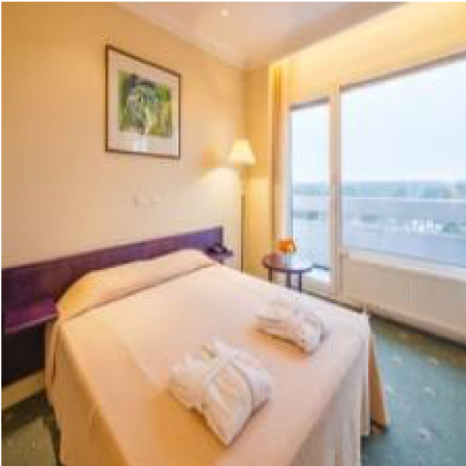
\includegraphics[width=.98\columnwidth]{figures/chapter5/data_augmentation/1.png}
        \caption{}
    \end{subfigure}
   \begin{subfigure}[b]{.19\columnwidth}
        \centering
        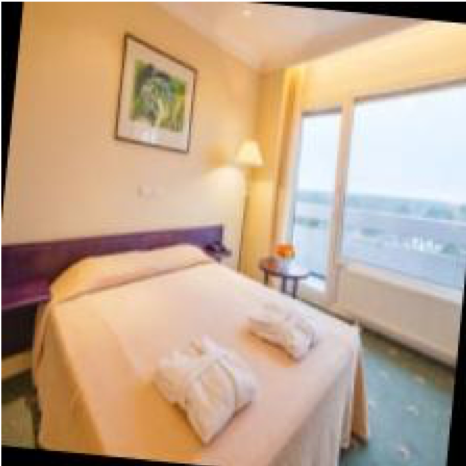
\includegraphics[width=.98\columnwidth]{figures/chapter5/data_augmentation/2.png}
        \caption{}
    \end{subfigure}
    \begin{subfigure}[b]{.19\columnwidth}
        \centering
        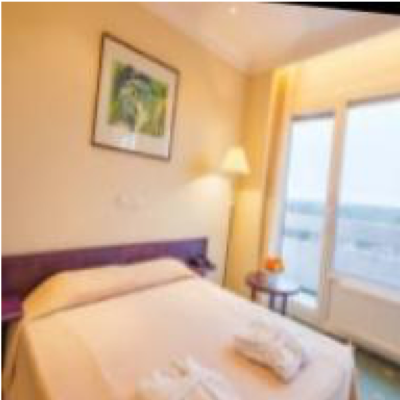
\includegraphics[width=.98\columnwidth]{figures/chapter5/data_augmentation/3.png}
        \caption{}
    \end{subfigure}
    \begin{subfigure}[b]{.19\columnwidth}
        \centering
        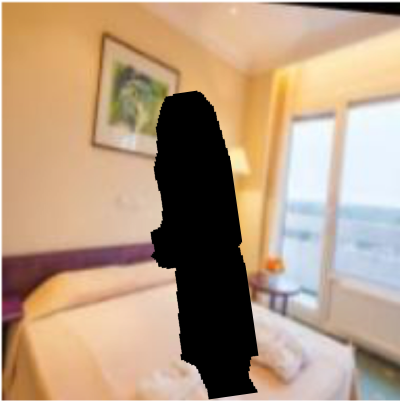
\includegraphics[width=.98\columnwidth]{figures/chapter5/data_augmentation/4.png}
        \caption{}
    \end{subfigure}
    \begin{subfigure}[b]{.19\columnwidth}
        \centering
        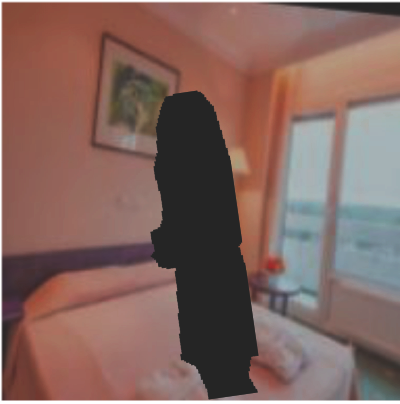
\includegraphics[width=.98\columnwidth]{figures/chapter5/data_augmentation/5.png}
        \caption{}
    \end{subfigure}
    \caption[Data augmentation to mimic properties of query images.]{Data augmentation steps to better match across different lighting conditions, scales and perspectives, and in the presence of large occlusions: (a) the original image; (b) after rotation; (c) after cropping; (d) after people mask applied; (e) after color filter rendered.}
    \label{fig:data_augmentation}
\end{figure}

Our method uses the Hotels-50K training set as input
to fine tune a Resnet-50 model, pre-trained for ImageNet, to output 256-D features. The training scheme is the  combinatorial variant of triplet loss described in~\cite{HermansBeyer2017Arxiv}.

In training, we balance the number of crowdsourced and travel website images in each batch. Additionally, we perform a set of data augmentation steps, highlighted in Figure~\ref{fig:data_augmentation}. Images from the batch are randomly selected and rotated between -35 and 35 degrees, cropped between 60\% and 100\% of the original size, modified with color and brightness, and masked with person shaped silhouettes, similar to process used for the test data. The set of masks applied in training do not overlap with those used to generated the Hotels-50K test data and will be made available. Training parameters
were selected using cross-validation. The final model
was fine-tuned for 65,000 iterations with 120 images per batch.

\subsection{Retrieval}
For retrieval, we compute feature representations
for all of the images in the Hotels-50K training set using
each method. Feature representations are also computed 
for each image in the test set, and the database images
a ranked via similarity to each test image using cosine similarity.

 \begin{table}
    \centering
      \begin{tabular}{c|ccc|}
      \multicolumn{1}{c}{} & \multicolumn{3}{c}{\textbf{Instance}} \\
      \cline{2-4}
      & K=1 & 10 & 100 \\
      \cline{1-4}
      \multicolumn{1}{|c|}{{\sc Fixed-Object}} & 0.8 & 0.9 & 1.3 \\
      \multicolumn{1}{|c|}{{\sc Fixed-Scene}} & 0.2 & 0.8 & 2.4\\
      \multicolumn{1}{|c|}{Ours} & \textbf{4.6} & \textbf{11.2} & \textbf{24.8} \\
      \cline{1-4}
      \multicolumn{4}{c}{} \\
      \multicolumn{1}{c}{} & \multicolumn{3}{c}{\textbf{Chain}} \\
      \cline{2-4}
      & K=1 & 3 & 5 \\
      \cline{1-4}
      \multicolumn{1}{|c|}{{\sc Fixed-Object}} & 5.0 & 29.0 & 79.2 \\
      \multicolumn{1}{|c|}{{\sc Fixed-Scene}} & 7.2 & 34.2 & 78.7\\
      \multicolumn{1}{|c|}{Ours} & \textbf{39.7} & \textbf{68.7} & \textbf{90.6} \\
      \cline{1-4}
      
      \end{tabular}
      \caption{Retrieval results by hotel instance and by hotel chain, reported as top-$K$ accuracy.}
      \label{tab:hotel_vs_chain_comparison}
\end{table}

\begin{table*}
    \centering
    \def\arraystretch{1.1}
    \begin{tabular}{l|ccc|ccc|ccc|ccc|ccc|}
        \multicolumn{1}{r}{\textbf{Occlusion:}}&\multicolumn{3}{c}{\textbf{none}} & \multicolumn{3}{c}{\textbf{low}} & \multicolumn{3}{c}{\textbf{medium}} & \multicolumn{3}{c}{\textbf{high}} \\
        \cline{2-13}
    %     & & 
    %     K=1 & 3 & 5 &
    %     1 & 3 & 5 & 
    %     1 & 3 & 5 & 
    %     1 & 3 & 5 \\
    %     \cline{2-14}
    %     \multirow{3}{*}{\raisebox{-.5\height}{\rotatebox{90}{Chain}}} & \multicolumn{1}{|l|}{{\sc Fixed-Object}} &
    %     5.0 & 29.0 & 79.2 &
    %     5.0 & 29.0 & 79.2 &
    %     5.0 & 29.0 & 79.2 & 
    %     5.0 & 29.0 & 79.2\\
    %     & \multicolumn{1}{|l|}{{\sc Fixed-Scene}} & 
    %     7.2 & 34.2 & 78.7 &
    %     7.2 & 34.2 & 78.7 & 
    %     7.2 & 34.2 & 78.7 & 
    %     7.2 & 34.1 & 78.7 \\
    %     & \multicolumn{1}{|l|}{Ours} & 
    %     \textbf{39.7} & \textbf{68.6}  & \textbf{90.6} & 
    %     \textbf{39.7} & \textbf{68.6}  & \textbf{90.6}  & 
    %     \textbf{39.7} & \textbf{68.6}  & \textbf{90.6}  & 
    %     \textbf{39.7} & \textbf{68.6}  & \textbf{90.6}  \\
    %     \cline{2-14}
    %     & \multicolumn{13}{c}{}
    % \\
    %     \cline{3-14}
        & K=1 & 10 & 100 &
        1 & 10 & 100 & 
        1 & 10 & 100 & 
        1 & 10 & 100 \\
        \cline{1-13}
        \multicolumn{1}{|l|}{{\sc Fixed-Object}} & 
        0.8 & 0.9 & 1.3 &
        0.3 & 0.4 & 0.7 & 
        0.0 & 0.0 & 0.0 & 
        0.0 & 0.1 & 0.4 \\
        \multicolumn{1}{|l|}{{\sc Fixed-Scene}} & 
        0.2 & 0.8 & 2.4 &
        0.1 & 0.5 & 1.9 & 
        0.1 & 0.4 & 1.5 & 
        0.0 & 0.1 & 1.0 \\
        \multicolumn{1}{|l|}{Ours} & 
        \textbf{4.6} & \textbf{11.2} & \textbf{24.8} &
        \textbf{4.1} & \textbf{10.4} & \textbf{23.9} & 
        \textbf{3.3} & \textbf{8.6} & \textbf{21.1} & 
        \textbf{2.3} & \textbf{6.5} & \textbf{17.1} \\
        \cline{1-13}
    \end{tabular}
    \caption{Image retrieval comparison reported as top-$K$ accuracy.}
    \label{tab:topK_accuracy}
\end{table*}

Table~\ref{tab:hotel_vs_chain_comparison} shows the image retrieval results by hotel instance and chain for all three methods. For all methods, the retrieval accuracy by hotel instance is significantly lower than the accuracy by hotel chain.  This is likely due to the difficulty discriminating between particular instances of hotel chains that look similar. The chain identification task is simple enough that even the fixed methods not fine-tuned to the task achieve
nearly 80\% top-5 accuracy on this task. Therefore, for our remaining
experiments, we focus on the more challenging problem to recognize a hotel instance.

Table~\ref{tab:topK_accuracy} shows the image retrieval results for all three methods for the test images with varying sizes of image masking. Our approach has significantly higher retrieval accuracy compared to the pre-trained approaches for all tests, both with and without occlusions.

\newcommand{\exResultsHeight}{.56in}
\newcommand{\queryImWidth}{.15\textwidth}
\begin{figure*}
\setlength{\tabcolsep}{1pt}
    \begin{tabular}{cccccccccccc}
    Query Image & Model & 1 & 2 & 3 & 4 & 5\\
    \cline{1-7}
        \multirow{3}{*}{\raisebox{-.75\height}{ 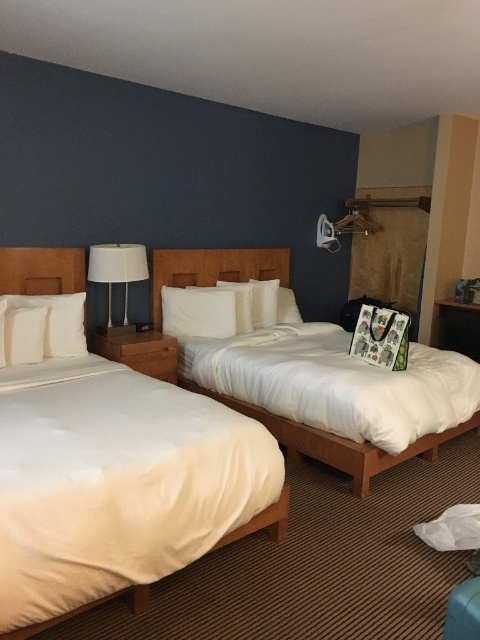
\includegraphics[width=\queryImWidth]{figures/chapter5/example_results/2/query.jpg}}}
        &
        \raisebox{-.5\height}{{\sc Fixed-Object}}
        & \raisebox{-.5\height}{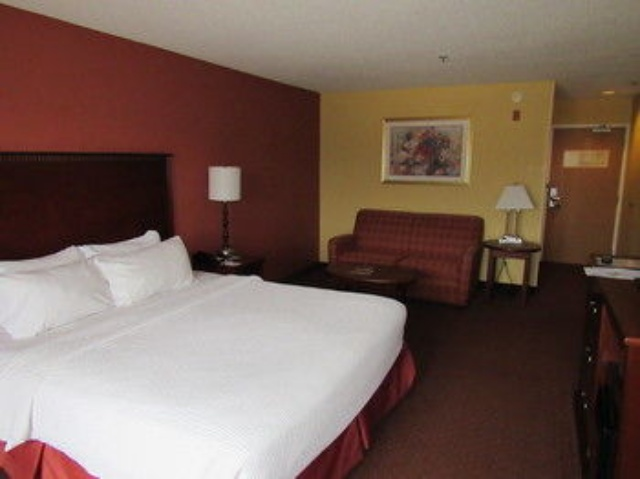
\includegraphics[height=\exResultsHeight]{figures/chapter5/example_results/2/ilsvrc/0_incorrect.jpg}}
        &\raisebox{-.5\height}{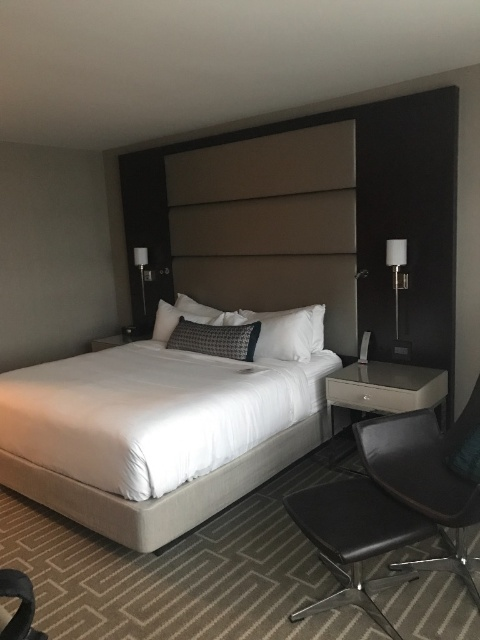
\includegraphics[height=\exResultsHeight]{figures/chapter5/example_results/2/ilsvrc/1_incorrect.jpg}}
        &\raisebox{-.5\height}{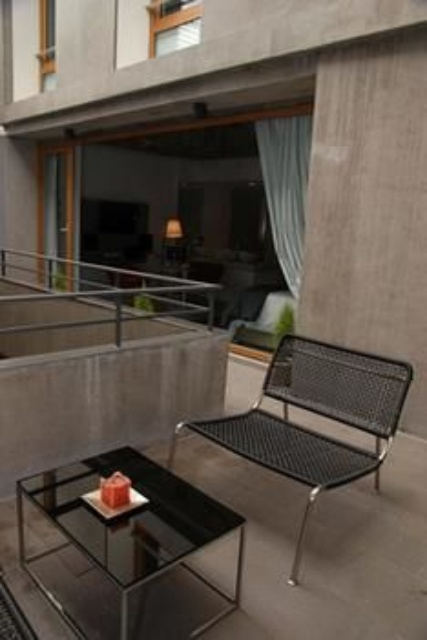
\includegraphics[height=\exResultsHeight]{figures/chapter5/example_results/2/ilsvrc/2_incorrect.jpg}}
        &\raisebox{-.5\height}{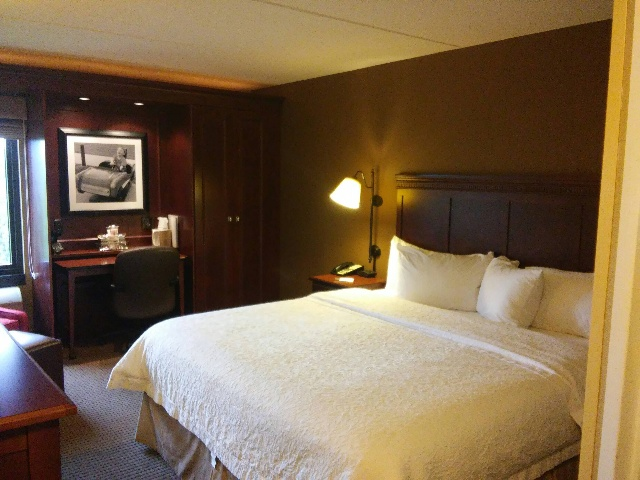
\includegraphics[height=\exResultsHeight]{figures/chapter5/example_results/2/ilsvrc/3_incorrect.jpg}}
        &\raisebox{-.5\height}{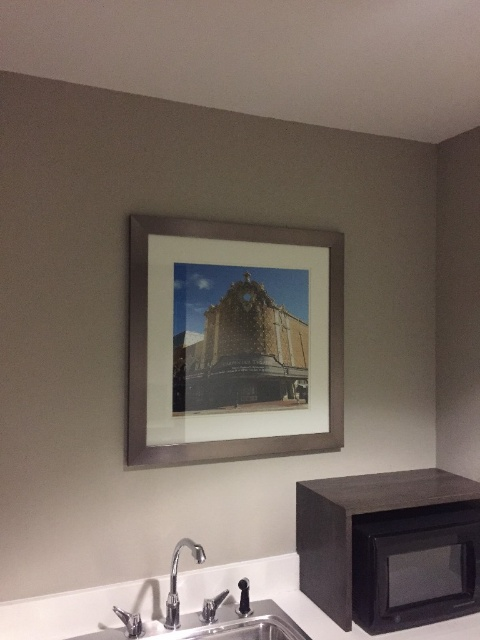
\includegraphics[height=\exResultsHeight]{figures/chapter5/example_results/2/ilsvrc/4_incorrect.jpg}}
    \\
    &
        \raisebox{-.5\height}{{\sc Fixed-Scene}}
        &\raisebox{-.5\height}{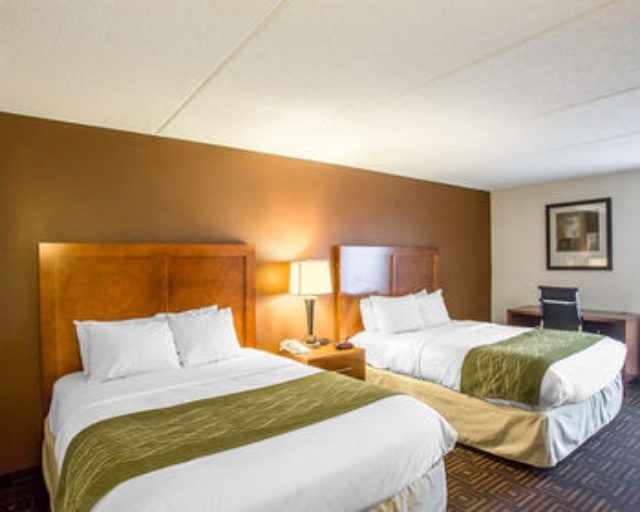
\includegraphics[height=\exResultsHeight]{figures/chapter5/example_results/2/places365/0_incorrect.jpg}}
        &\raisebox{-.5\height}{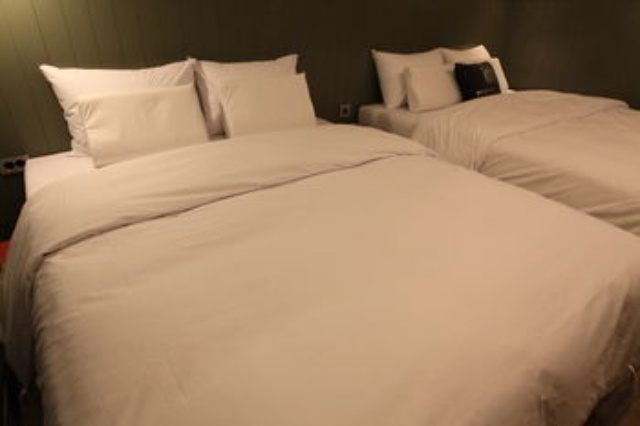
\includegraphics[height=\exResultsHeight]{figures/chapter5/example_results/2/places365/1_incorrect.jpg}}
        &\raisebox{-.5\height}{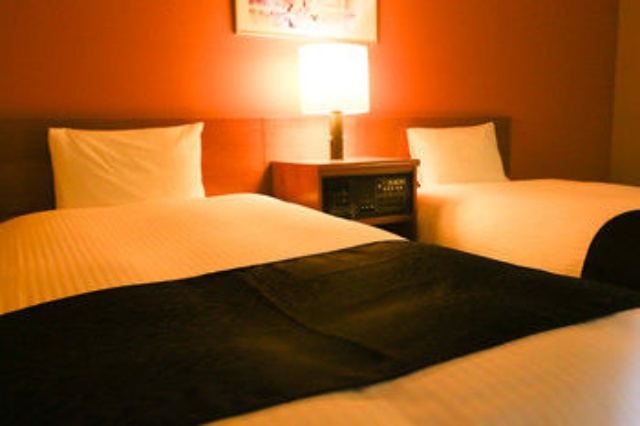
\includegraphics[height=\exResultsHeight]{figures/chapter5/example_results/2/places365/2_incorrect.jpg}}
        &\raisebox{-.5\height}{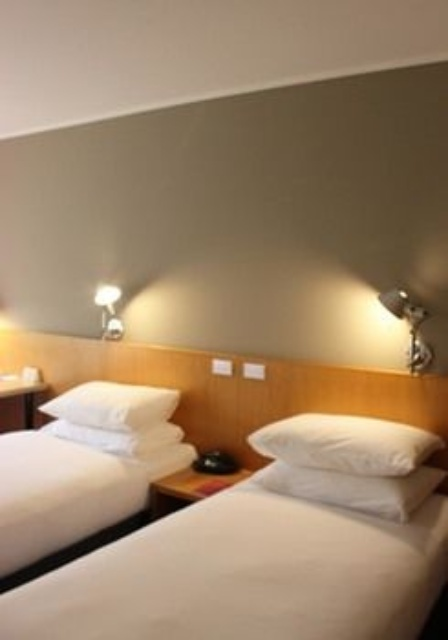
\includegraphics[height=\exResultsHeight]{figures/chapter5/example_results/2/places365/3_incorrect.jpg}}
        &\raisebox{-.5\height}{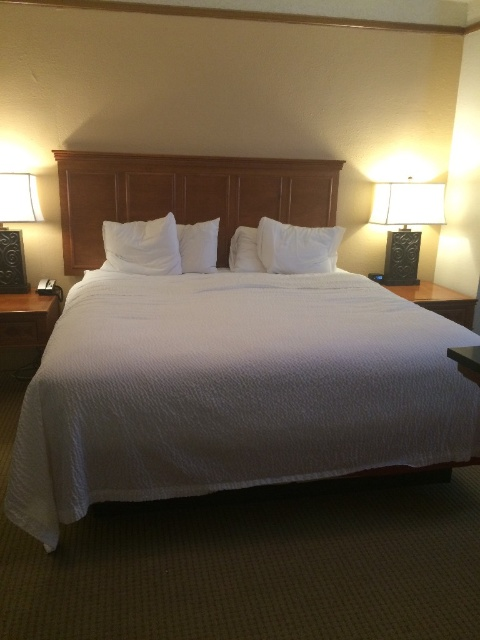
\includegraphics[height=\exResultsHeight]{figures/chapter5/example_results/2/places365/4_incorrect.jpg}}
    \\
    &
        \raisebox{-.5\height}{Ours}
        & \raisebox{-.5\height}{\fcolorbox{green}{green}{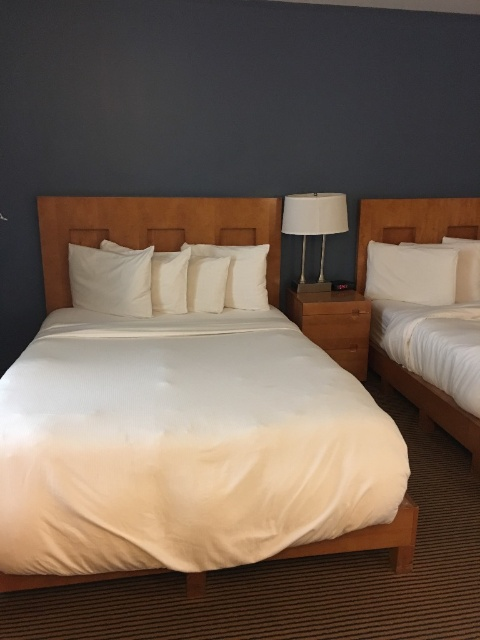
\includegraphics[height=\exResultsHeight]{figures/chapter5/example_results/2/ours/0_correct.jpg}}}
        &\raisebox{-.5\height}{\fcolorbox{green}{green}{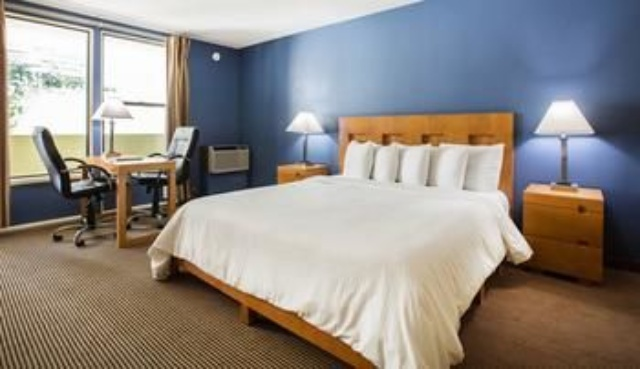
\includegraphics[height=\exResultsHeight]{figures/chapter5/example_results/2/ours/1_correct.jpg}}}
        &\raisebox{-.5\height}{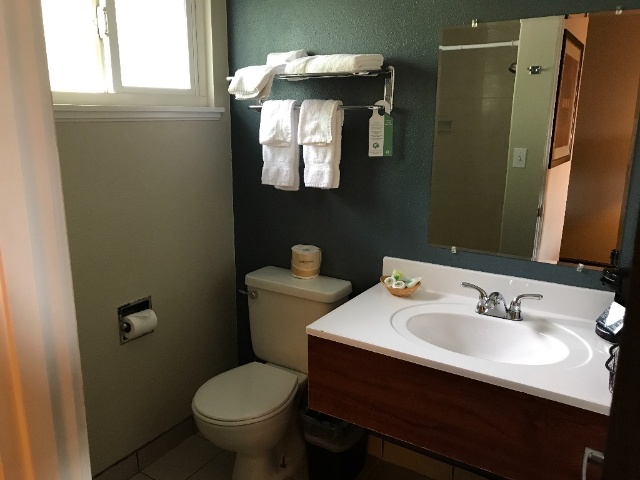
\includegraphics[height=\exResultsHeight]{figures/chapter5/example_results/2/ours/2_incorrect.jpg}}
        &\raisebox{-.5\height}{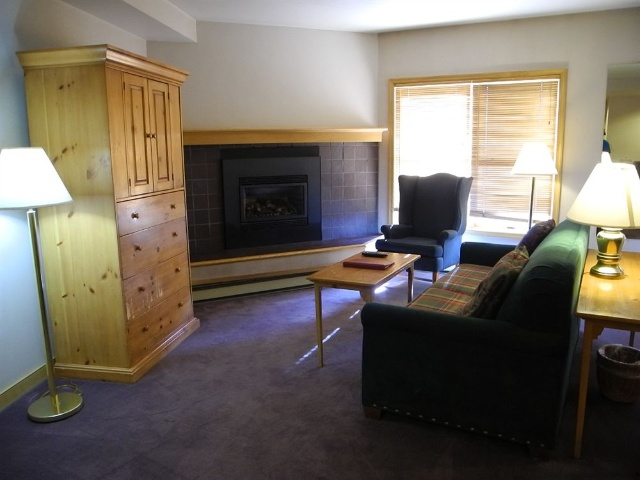
\includegraphics[height=\exResultsHeight]{figures/chapter5/example_results/2/ours/3_incorrect.jpg}}
        & \raisebox{-.5\height}{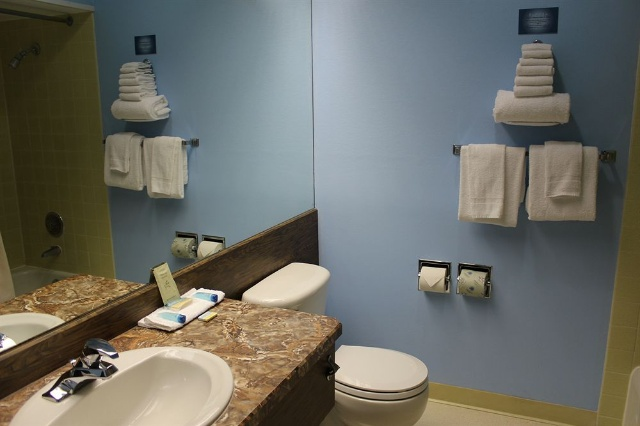
\includegraphics[height=\exResultsHeight]{figures/chapter5/example_results/2/ours/4_incorrect.jpg}}\\
    \cline{1-7}
    
    \multirow{3}{*}{\raisebox{-1.2\height}{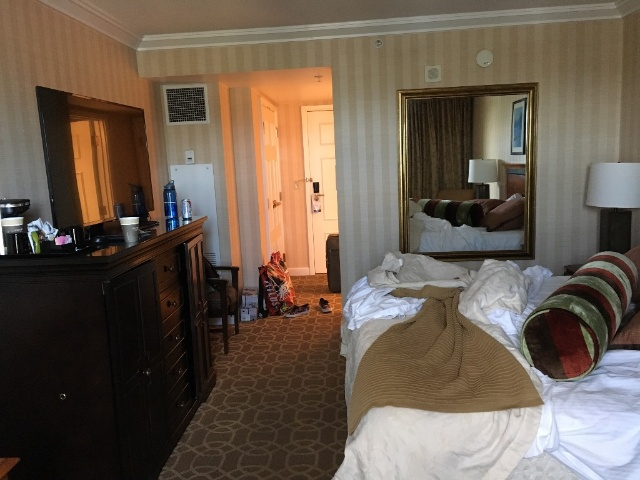
\includegraphics[width=\queryImWidth]{figures/chapter5/example_results/3/query.jpg}}}
        &\raisebox{-.5\height}{{\sc Fixed-Object}}
        & \raisebox{-.5\height}{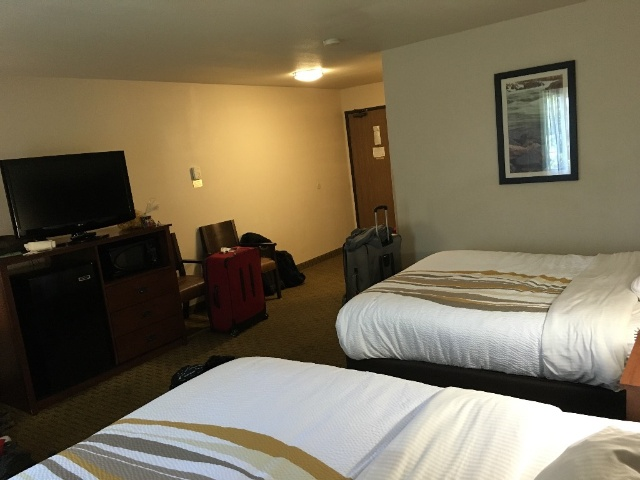
\includegraphics[height=\exResultsHeight]{figures/chapter5/example_results/3/ilsvrc/0_incorrect.jpg}}
        &\raisebox{-.5\height}{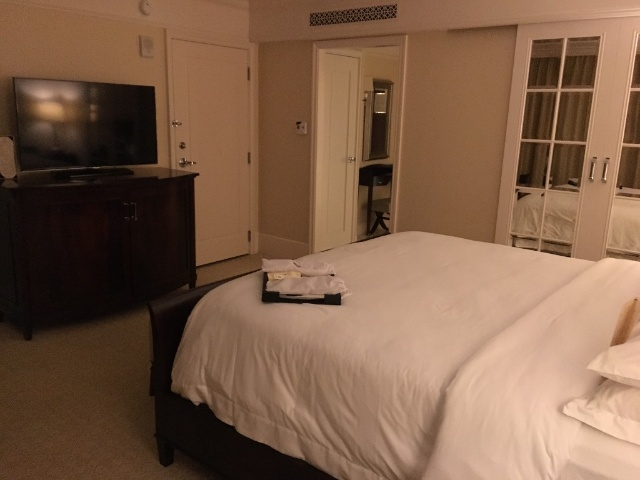
\includegraphics[height=\exResultsHeight]{figures/chapter5/example_results/3/ilsvrc/1_incorrect.jpg}}
        &\raisebox{-.5\height}{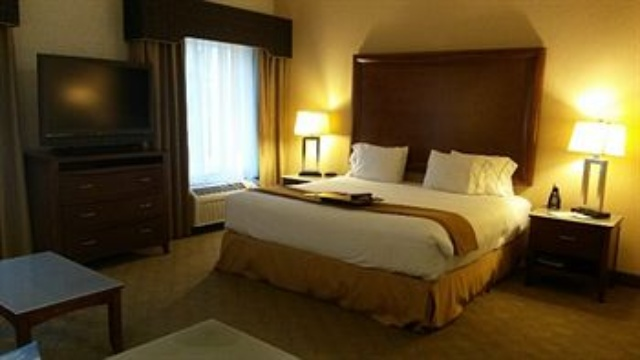
\includegraphics[height=\exResultsHeight]{figures/chapter5/example_results/3/ilsvrc/2_incorrect.jpg}}
        &\raisebox{-.5\height}{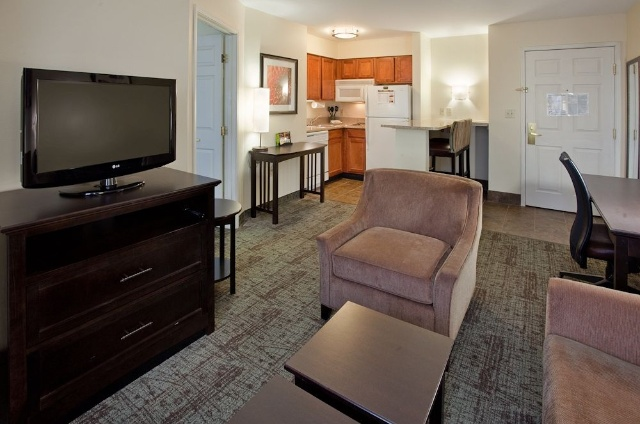
\includegraphics[height=\exResultsHeight]{figures/chapter5/example_results/3/ilsvrc/3_incorrect.jpg}}
        &\raisebox{-.5\height}{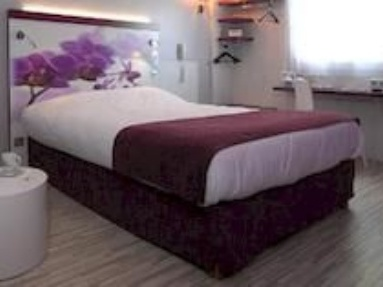
\includegraphics[height=\exResultsHeight]{figures/chapter5/example_results/3/ilsvrc/4_incorrect.jpg}}
    \\
     &
        \raisebox{-.5\height}{{\sc Fixed-Scene}}
        &\raisebox{-.5\height}{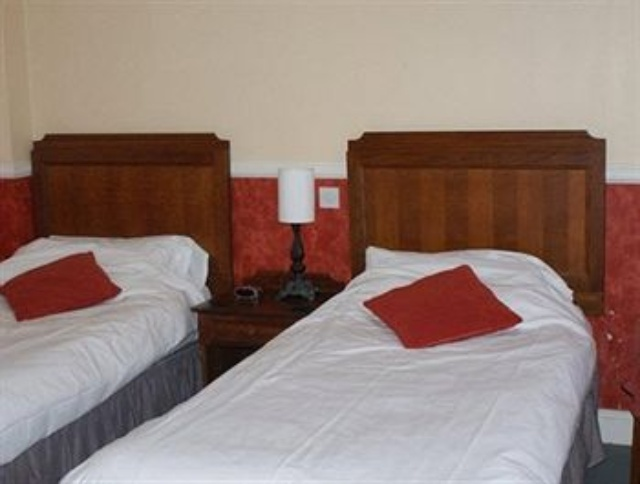
\includegraphics[height=\exResultsHeight]{figures/chapter5/example_results/3/places365/0_incorrect.jpg}}
        &\raisebox{-.5\height}{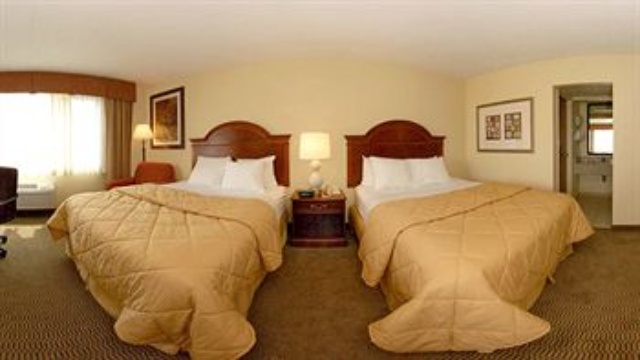
\includegraphics[height=\exResultsHeight]{figures/chapter5/example_results/3/places365/1_incorrect.jpg}}
        &\raisebox{-.5\height}{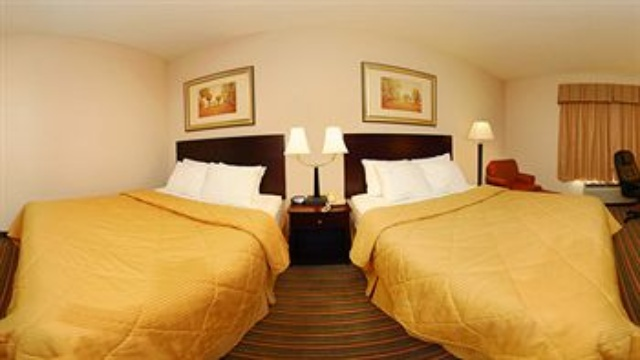
\includegraphics[height=\exResultsHeight]{figures/chapter5/example_results/3/places365/2_incorrect.jpg}}
        &\raisebox{-.5\height}{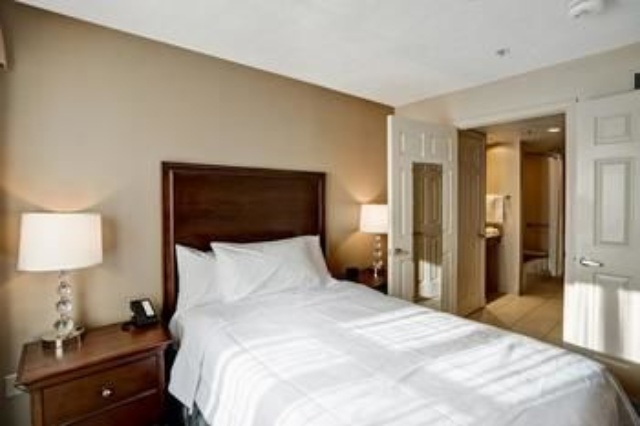
\includegraphics[height=\exResultsHeight]{figures/chapter5/example_results/3/places365/3_incorrect.jpg}}
        &\raisebox{-.5\height}{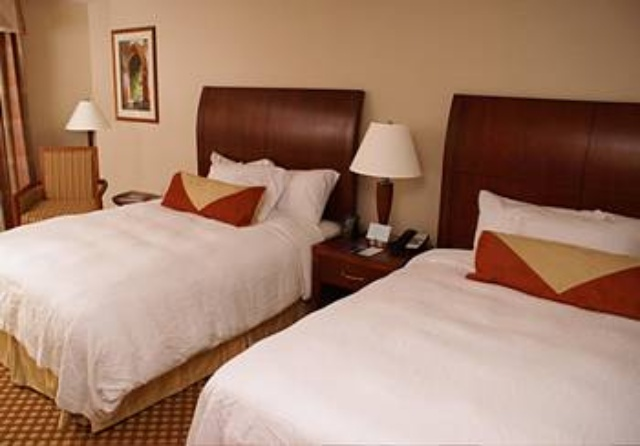
\includegraphics[height=\exResultsHeight]{figures/chapter5/example_results/3/places365/4_incorrect.jpg}}
    \\
    &
        \raisebox{-.5\height}{Ours}
        & \raisebox{-.5\height}{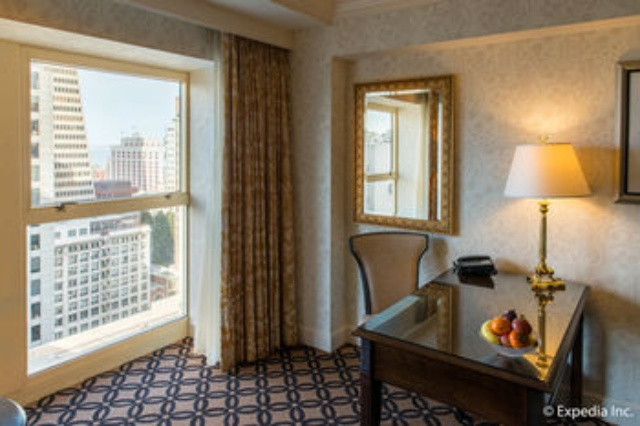
\includegraphics[height=\exResultsHeight]{figures/chapter5/example_results/3/ours/0_incorrect.jpg}}
        &\raisebox{-.5\height}{\fcolorbox{green}{green}{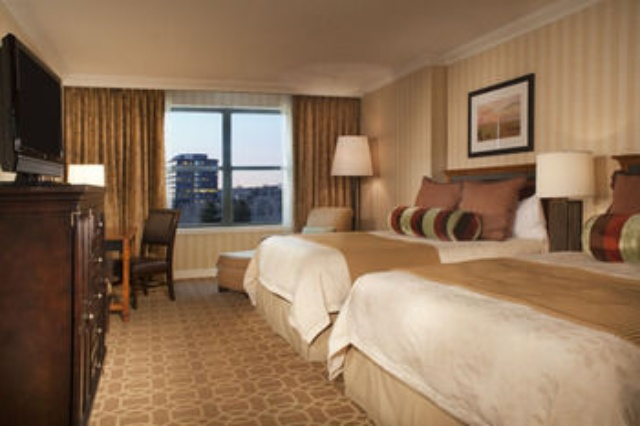
\includegraphics[height=\exResultsHeight]{figures/chapter5/example_results/3/ours/1_correct.jpg}}}
        &\raisebox{-.5\height}{\fcolorbox{green}{green}{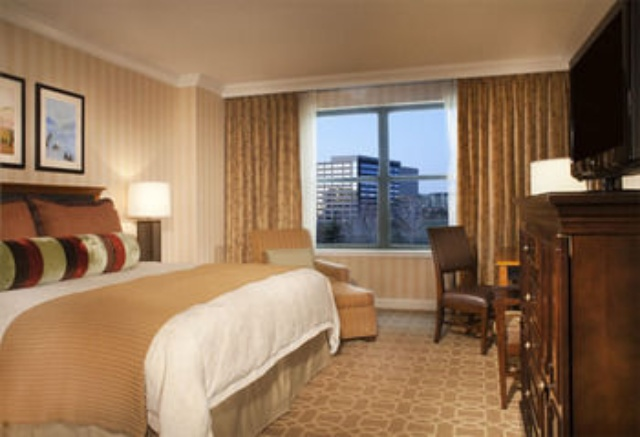
\includegraphics[height=\exResultsHeight]{figures/chapter5/example_results/3/ours/2_correct.jpg}}}
        &\raisebox{-.5\height}{\fcolorbox{green}{green}{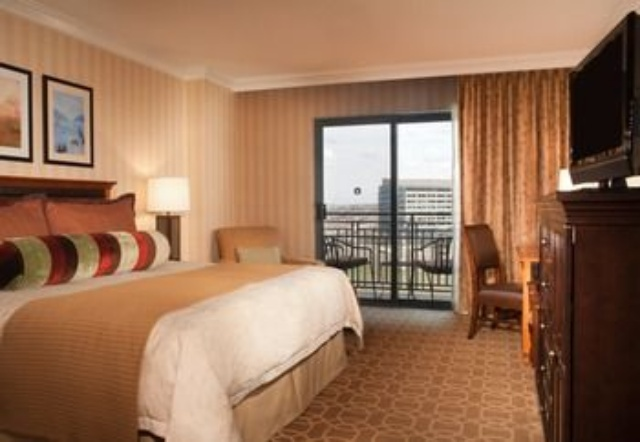
\includegraphics[height=\exResultsHeight]{figures/chapter5/example_results/3/ours/3_correct.jpg}}}
        & \raisebox{-.5\height}{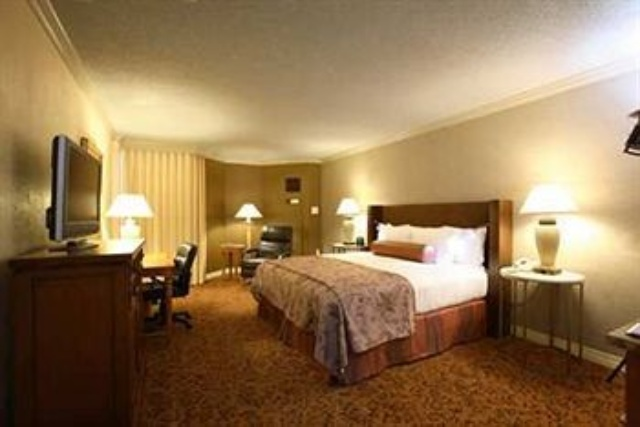
\includegraphics[height=\exResultsHeight]{figures/chapter5/example_results/3/ours/4_incorrect.jpg}}\\
        
    \cline{1-7}  
    \multirow{3}{*}{\raisebox{-1.2\height}{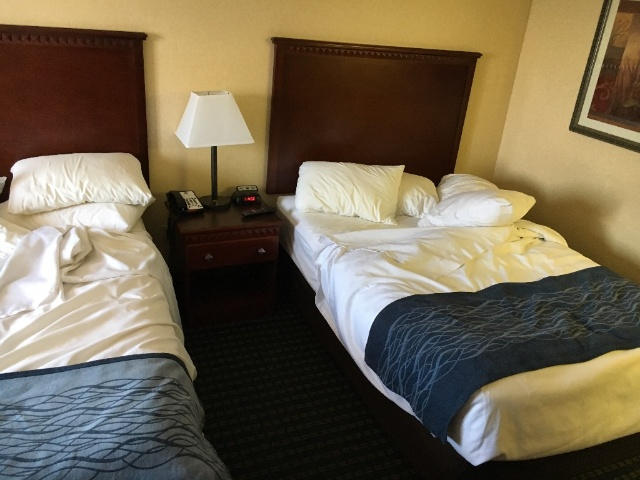
\includegraphics[width=\queryImWidth]{figures/chapter5/example_results/4/query.jpg}}}
        &\raisebox{-.5\height}{{\sc Fixed-Object}}
        & \raisebox{-.5\height}{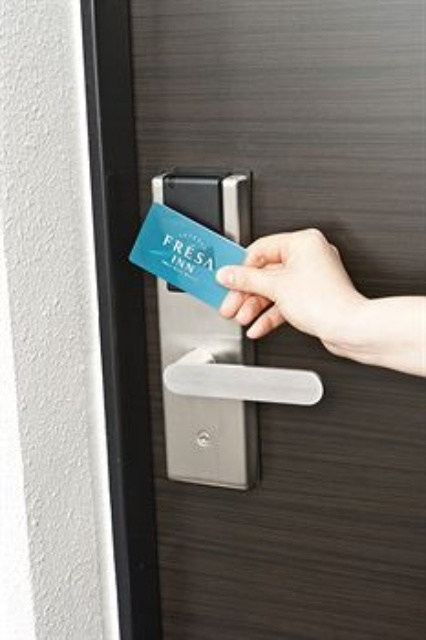
\includegraphics[height=\exResultsHeight]{figures/chapter5/example_results/4/ilsvrc/0_incorrect.jpg}}
        &\raisebox{-.5\height}{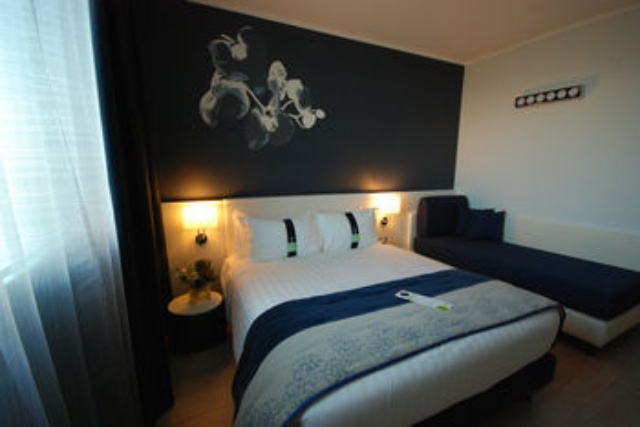
\includegraphics[height=\exResultsHeight]{figures/chapter5/example_results/4/ilsvrc/1_incorrect.jpg}}
        &\raisebox{-.5\height}{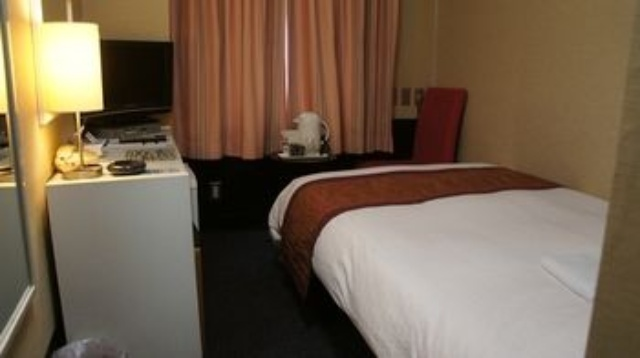
\includegraphics[height=\exResultsHeight]{figures/chapter5/example_results/4/ilsvrc/2_incorrect.jpg}}
        &\raisebox{-.5\height}{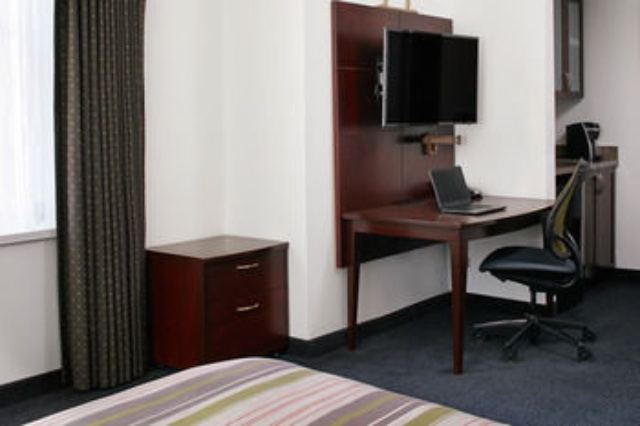
\includegraphics[height=\exResultsHeight]{figures/chapter5/example_results/4/ilsvrc/3_incorrect.jpg}}
        &\raisebox{-.5\height}{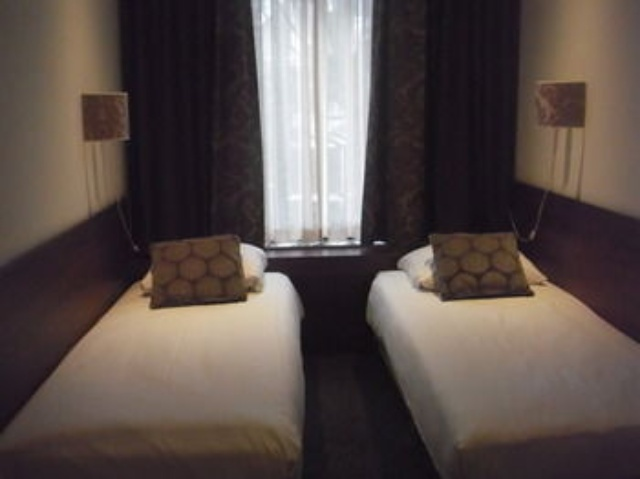
\includegraphics[height=\exResultsHeight]{figures/chapter5/example_results/4/ilsvrc/4_incorrect.jpg}}
    \\
        &
        \raisebox{-.5\height}{{\sc Fixed-Scene}}
        &\raisebox{-.5\height}{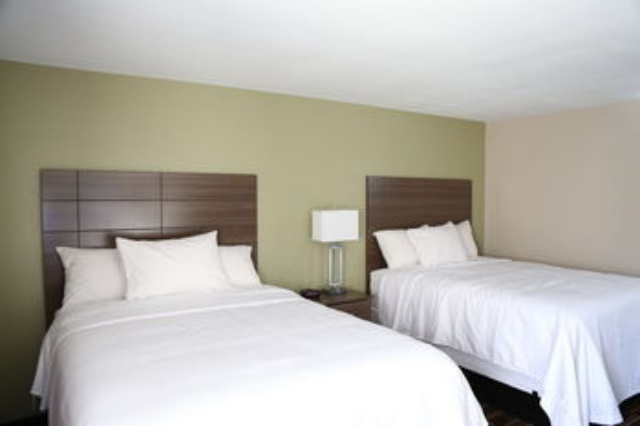
\includegraphics[height=\exResultsHeight]{figures/chapter5/example_results/4/places365/0_incorrect.jpg}}
        &\raisebox{-.5\height}{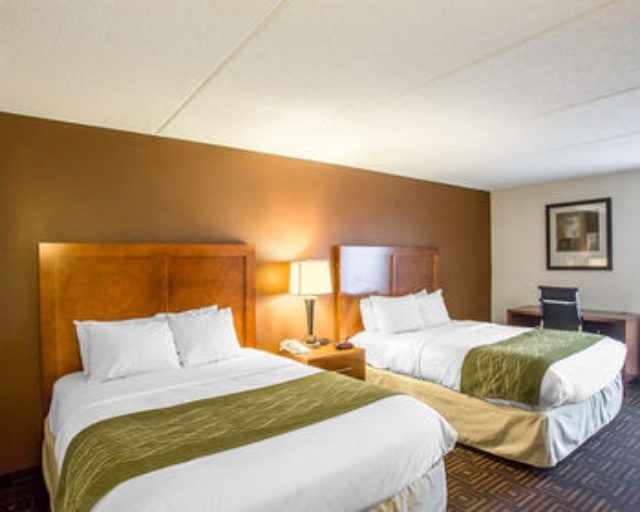
\includegraphics[height=\exResultsHeight]{figures/chapter5/example_results/4/places365/1_incorrect.jpg}}
        &\raisebox{-.5\height}{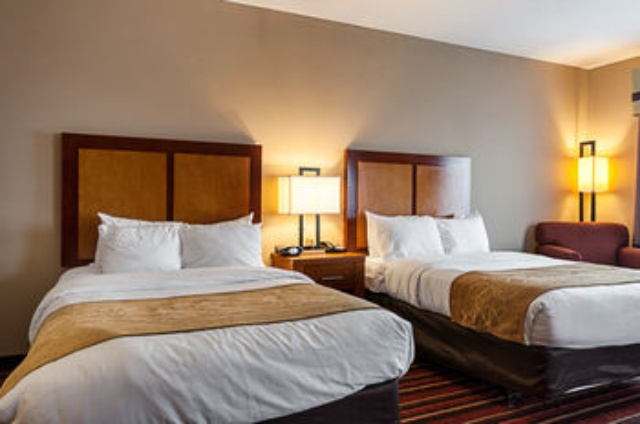
\includegraphics[height=\exResultsHeight]{figures/chapter5/example_results/4/places365/2_incorrect.jpg}}
        &\raisebox{-.5\height}{\includegraphics[height=\exResultsHeight]{figures/chapter5/example_results/4/places365/3_incorrect.jpg}}
        &\raisebox{-.5\height}{\includegraphics[height=\exResultsHeight]{figures/chapter5/example_results/4/places365/4_incorrect.jpg}}
    \\
        &
        \raisebox{-.5\height}{Ours}
        & \raisebox{-.5\height}{\includegraphics[height=\exResultsHeight]{figures/chapter5/example_results/4/ours/0_incorrect.jpg}}
        &\raisebox{-.5\height}{\includegraphics[height=\exResultsHeight]{figures/chapter5/example_results/4/ours/1_incorrect.jpg}}
        &\raisebox{-.5\height}{\includegraphics[height=\exResultsHeight]{figures/chapter5/example_results/4/ours/2_incorrect.jpg}}
        &\raisebox{-.5\height}{\includegraphics[height=\exResultsHeight]{figures/chapter5/example_results/4/ours/3_incorrect.jpg}}
        & \raisebox{-.5\height}{\fcolorbox{green}{green}{\includegraphics[height=\exResultsHeight]{figures/chapter5/example_results/4/ours/4_correct.jpg}}}\\
    \end{tabular}
    \caption{The top 5 most similar results for the models trained on the Places-365 dataset, the ILSVRC dataset, and our model trained on travel website and TraffickCam images with data augmentation. Images from the correct hotel instance are highlighted in green.}
    \label{fig:top5_results}
\end{figure*}


Figure~\ref{fig:top5_results} shows the top 5 results for several query images using {\sc Fixed-Object}, {\sc Fixed-Scene} and our approaches.  Unlike {\sc Fixed-Object} and {\sc Fixed-Scene}, our model appears to encode information about the important colors and objects in a hotel room. In the top example in Figure~\ref{fig:top5_results}, our approach finds examples from the correct hotel, as well as other images with similar blue walls and headboards. Our model also performs reasonably well even in the case where there is large amounts of clutter in the query image, as seen in the middle example in Figure~\ref{fig:top5_results}. The last example in Figure~\ref{fig:top5_results} highlights the difficulty of hotel instance recognition given the similarity between instances of the same hotel chain -- nearly all of the top images retrieved by our are from the correct hotel chain, but
not necessarily the correct hotel. 

\subsection{Classification}
For the classification task, we adapt the image
embedding approaches used for image retrieval to report class posterior probabilities. For each method for each test image, 
we find the 100 most similar images in the database 
using cosine similarity between the output features. The proportion of each class (hotel instance or hotel chain)
in the resulting set is the Bayesian estimate of the posterior probability.


\begin{table}
    \def\arraystretch{1.1}
    \centering
    \begin{tabular}{c|c|c|c|c|}
        \multicolumn{1}{r}{\textbf{Occlusion:}} & \multicolumn{1}{c}{\textbf{none}} & \multicolumn{1}{c}{\textbf{low}} & \multicolumn{1}{c}{\textbf{medium}} & \multicolumn{1}{c}{\textbf{high}} \\
        \cline{1-5}
        \multicolumn{1}{|l|}{{\sc Fixed-Object}} & 34.1 & 34.3 & 34.5 & 34.4 \\
        \multicolumn{1}{|l|}{{\sc Fixed-Scene}} & 33.8 & 33.9 & 34.1 & 34.2 \\
        \multicolumn{1}{|l|}{Ours} & \textbf{27.0} & \textbf{27.2}  & \textbf{28.1} & \textbf{29.3} \\
        \cline{1-5}
    \end{tabular}
    \caption{Multi-class log loss for
    each method on the hotel instance classification task. }
    \label{tab:log_loss}
\end{table}

Table~\ref{tab:log_loss} shows the multiclass log loss for each method for varying levels of occlusions in the test images. 
In all cases, our approach outperforms features from the pretrained models. However, there is still significant room 
for improved performance for both hotel instance and hotel chain classification. 

\subsection{Ablation Study}
To quantify the effects of both the Hotels-50K data and
augmentation steps in our approach, we compare the
results of variants of our method on the hotel instance
retrieval task with and without significant occlusions.

%\setlength{\tabcolsep}{4pt}
\begin{table}
    %\def\arraystretch{1.1}
    \centering
    %   \begin{tabular}{c|ccc|}
    %     \multicolumn{1}{c}{} & \multicolumn{3}{c}{\textbf{no occlusions}} \\
    %     \cline{2-4}
    %     \multicolumn{1}{c|}{\textbf{Model}} & K=1 & 3 & 5 \\
    %     \cline{1-4}
    %     \multicolumn{1}{|c|}{Method$_1$} & 27.3 & 59.1 & 90.9 \\
    %     \multicolumn{1}{|c|}{Method$_2$} & 39.5 & 67.5 & 89.3\\
    %     \multicolumn{1}{|c|}{Method$_3$} & \textbf{39.7} & \textbf{68.6} & \textbf{90.6}\\
    %     \cline{1-4}
    %     \multicolumn{4}{c}{}\\
    %     \multicolumn{4}{c}{(b) By hotel chain.}
    % \end{tabular}
    % \quad
    \begin{tabular}{c|ccc|ccc|}
        \multicolumn{1}{r}{\textbf{Occlusion:}} & \multicolumn{3}{c}{\textbf{none}} & \multicolumn{3}{c}{\textbf{medium}} \\
        \cline{2-7}
        \multicolumn{1}{c|}{} & K=1 & 10 & 100 & 1 & 10 & 100 \\
        \cline{1-7}
        \multicolumn{1}{|l|}{Ours -A,-I} & 2.6 & 5.5 & 12.4 & 0.8 & 2.2 & 5.9\\
        \multicolumn{1}{|l|}{Ours -A} & \textbf{4.6} & 11.2 & \textbf{25.5} & 1.7 & 5.2 & 15.0 \\
        \multicolumn{1}{|l|}{Ours} & \textbf{4.6} & \textbf{11.7} & 24.8 & \textbf{3.3} & \textbf{8.6} & \textbf{21.1}\\
        \cline{1-7}
    \end{tabular}
    
    \caption{Ablation study reported as top-$K$ hotel instance retrieval for our method and variants without data augmentation (-A) and without crowdsourced images (-I).}
    \label{tab:ablationStudy}
\end{table}

Table~\ref{tab:ablationStudy} shows the results
for the ablation experiment. We evaluate our approach
without the data augmentation steps and additionally 
without including the crowdsourced images, which are those most similar to the real-world images. The inclusion of the crowdsourced images has a significant impact on the performance both with and without occlusions in the test image. The data augmentation steps do not have an impact on the performance in the occluded cases, but in the medium occlusion case, which roughly corresponds to sizes of the masked regions in real-world cases, the benefits of the data augmentation steps are apparent, increasing the top-$K$ accuracy by more than 50\% for $K=10$.